% Document class for LME theses: lmedoc
% %LANGUAGE
% %CONFIG
%    The option "german" uses german.sty
%    For english papers, use the "english" option
% Possible types of theses:
% bt - Bachelor's thesis
% mt - Master's thesis
% diss - Dissertation
% sa - Student thesis
% fp - Forschungspraktikum
% pa - Projektarbeit
%\documentclass[german,bt]{lmedoc/lmedoc}
\documentclass[english,fp]{lmedoc/lmedoc}


%%%%%%%%%%%%%%%%%%
% pdflatex and lualatex are supported
% ++ "Umlaut" support
%    The package "inputenc" can be used to write Umlaute or the german double s
%    directly. You need to use the correct encoding, e.g. latin1.
\usepackage{iftex}
\ifPDFTeX
  \usepackage[utf8]{inputenc}
  \usepackage[T1]{fontenc}
  \usepackage{lmodern}
\else
  \ifXeTeX
     \usepackage{fontspec}
  \else 
     \usepackage{luatextra}
  \fi
\fi

%Load additional packages
\usepackage{lmedoc/packages}
% put in this file your abbreviations
% add your abbreviations here
\newabbreviation{ato}{ATO}{Automatic Train Operation}
\newabbreviation{cnn}{CNN}{Convolutional Neural Network}
\newabbreviation{hsv}{HSV}{Hue, Saturation, and Value}
\newabbreviation{iou}{IoU}{Intersection over Union}
\newabbreviation{kit}{KIT}{Karlsruhe Institute of Technology}
\newabbreviation{map}{mAP}{mean Average Precision}
\newacronym{nms}{NMS}{Non-Maximum Suppression}
\newabbreviation{sahi}{SAHI}{Slicing Aided Hyper Inference}
\newabbreviation{svm}{SVM}{Support Vector Machine}
\newabbreviation{vit}{ViT}{Vision Transformer}
\newabbreviation{yolo}{YOLO}{You Only Look Once}

%%%%%%%%%%%%%%%%%%%%%%%%%%%%

% supress messages because of underful hbox, this is not a problem
\hbadness=10000



% some useful commands
\makeatletter % let's define a single dot
\DeclareRobustCommand\onedot{\futurelet\@let@token\@onedot}
\newcommand{\@onedot}{\ifx\@let@token.\else.\null\fi\xspace}
\makeatother



% Sets the bib file

\addbibresource{literature.bib}

% When writing a large document, it is sometimes useful to work on selected sections of the document.
% Use this command to only build the document partially. Speeds up the developement cycle.
% For the final product, this has to be commented out.
%\includeonly{introduction,appendix,foo,bar}

% Cover variables for easy editing
\newcommand{\ReportTitle}{RAIL-BENCH Object Detection Challenge}
\newcommand{\ReportDocumentType}{Project Report}
\newcommand{\ReportMembers}{%
  \begin{tabular}{@{}lll@{}}
    \textbf{Forename} & \textbf{Surname} & \textbf{Student number} \\
    Forename 1 & Surname 1 & Student number 1 \\
    Forename 2 & Surname 2 & Student number 2 \\
  \end{tabular}%
}
\newcommand{\ReportAdvisor}{Advisor}
\newcommand{\ReportStart}{Start}
\newcommand{\ReportEnd}{End}

\makeatletter
\def\enddeckblatt{%
\clearpage
\thispagestyle{empty}
\vspace*{-4cm}
\begin{flushleft}
\begin{tabular}{@{} c @{\hspace{6cm}} c @{}}
\adjustbox{valign=t}{
\includegraphics[width=5.5cm]{lmedoc/FAU_TechFak_EN_H_RGB_darkblue-1.png}} & \adjustbox{valign=t}{
\includegraphics[width=5.5cm]{lmedoc/logo_large.png}}
\end{tabular}
\end{flushleft}
\vspace*{1.6cm}
\begin{center}
\Large
{\bfseries \@Titel}\\[20mm]
\large
{\bfseries \ReportDocumentType}\\[10mm]
\normalsize
\ifnum\language=\l@english submitted \else vorgelegt \fi \\
\ifnum\language=\l@english by \else von \fi \\
\vskip 0.8cm plus 0.2cm minus 0.5cm\relax
\end{center}
\begin{center}
\ReportMembers\\[4mm]
\vfill
\end{center}
\begin{center}
\ifnum\language=\l@english\relax
  Written at
\else
  Angefertigt am
\fi
\\[5mm]
Lehrstuhl f"ur Mustererkennung (Informatik 5)\\
Department Informatik \\
Friedrich-Alexander-Universit"at Erlangen-N"urnberg.\\[5mm]
\@ifundefined{ZweitInstitut}{}{%
\ifnum\language=\l@english\relax
  in Cooperation with
\else
  in Zusammenarbeit mit
\fi
\\[5mm]
  \ZweitInstitut\\[10mm]
}
\end{center}
\begin{flushleft}
\ifnum\language=\l@english\relax Advisor\else Betreuer\fi: \@Betreuer \\[2mm]
\ifnum\language=\l@english\relax Started\else Beginn der Arbeit\fi: \@Start \\[2mm]
\ifnum\language=\l@english\relax Finished\else Abgabe der Arbeit\fi: \@Ende \\
\end{flushleft}
\clearpage
\egroup}
\makeatother


\pagenumbering{roman}

\begin{document}
\clearpage
% %CONFIG
% This is for students' theses
  \begin{deckblatt}
    \Titel{\ReportTitle} % Title
    \Name{} % Last name (unused in custom cover)
    \Vorname{} % Given name (unused in custom cover)
    \Geburtsort{} % Place of birth (not used)
    \Geburtsdatum{} % Date of birth (not used)
    \Betreuer{\ReportAdvisor} % Advisor
    \Start{\ReportStart} % Start date
    \Ende{\ReportEnd} % End date
    %\ZweitInstitut{ZweitInstitut} % Cooperation partner
  \end{deckblatt}


\cleardoublepage
% Only necessary for thesis

Ich versichere, dass ich die Arbeit ohne fremde Hilfe und ohne Benutzung
anderer als der angegebenen Quellen angefertigt habe und dass die Arbeit
in gleicher oder "ahnlicher Form noch keiner anderen Pr"ufungsbeh"orde
vorgelegen hat und von dieser als Teil einer Pr"ufungsleistung
angenommen wurde. Alle Ausf"uhrungen, die w"ortlich oder sinngem"a"s
"ubernommen wurden, sind als solche gekennzeichnet.
\\


\cleardoublepage


\begin{center}
\bfseries
% Abstract in German
{\selectlanguage{german}"Ubersicht"}
\normalfont
\end{center}


\vspace{5.0cm}

\begin{center}
\bfseries
% Abstract in English
{\selectlanguage{english}Abstract}
\normalfont
\end{center}


\cleardoublepage

\tableofcontents

\cleardoublepage \pagenumbering{arabic}

% Report structure
\chapter{Introduction}
\label{ch:introduction}

Modern railway systems are undergoing a profound transformation driven by increased traffic volumes, rising safety expectations, and long-term ambitions toward automated and driverless train operation. As highlighted in the RAIL-BENCH kickoff presentation, demographic changes, strong competition from other transportation modes, and the growing demand for both passenger and freight transport intensify the need for reliable perception systems capable of supporting future \acrfull{ato} scenarios. Many of the tasks traditionally performed by human drivers - including obstacle recognition, signal interpretation, and track infrastructure monitoring - are fundamental perception tasks that must be replicated by technical systems to enable safe autonomous operation. Deep learning has demonstrated remarkable progress in visual perception, yet its application in the railway domain remains limited by the scarcity of publicly available datasets. The lack of standardized evaluation protocols also prevents a fair comparison between different methods. \cite{railbench-kickoff}


As explained by Bätz et al.~\cite{railbench-object-paper}, a particular challenge arises from the nature of existing railway infrastructure.
While automated operation has already been successfully established in isolated environments such as metro systems and people movers, these systems operate on infrastructure where access to the tracks is inherently restricted and the track occupancy can be reliably controlled. In contrast, conventional railway networks frequently include level crossings, open platform areas and shared-traffic environments, making it impossible to assume that the track is free of obstacles at all times. To address these challenges, \acrfull{kit} has introduced \emph{RAIL-BENCH}, the first benchmark suite dedicated to perception tasks in railway environments. RAIL-BENCH provides open datasets, unified evaluation metrics, and clearly defined testing procedures to facilitate fair comparisons between methods and accelerate research and development in this safety-critical domain \cite{railbench-object-paper}. RAIL-BENCH supports five scientific challenges \cite{railbench-object-paper}:
\begin{itemize}
    \item Rail Track Detection
    \item Object Detection
    \item Vegetation Segmentation
    \item Multiple Object Tracking
    \item Monocular Visual Odometry
\end{itemize}

Among the five challenges included in the suite, the \emph{RAIL-BENCH Object Detection Challenge} focuses on detecting and classifying objects relevant to railway operation. This challenge is built upon a dataset of 2500 real-world RGB images recorded from a train driver's perspective under diverse environmental conditions, including urban, rural, and station scenarios, and varying weather and camera setups \cite{railbench-object-detection-page}. Each image is annotated with axis-aligned bounding boxes covering seven object categories \cite{railbench-object-detection-page}:
\begin{itemize}
    \item Train
    \item Person
    \item Bicycle
    \item Road Vehicle
    \item Signal
    \item Signal Pole
    \item Catenary Pole
\end{itemize}
Additional annotation attributes such as occlusion levels and ignore flags further reflect the complexity of real railway scenes, where small, distant, or densely grouped objects frequently occur.

The challenge evaluates submitted predictions using the COCO-style \acrfull{map} across multiple \acrfull{iou} thresholds. Three difficulty levels - easy, moderate, and hard - are defined based on bounding box size and occlusion, with final rankings determined by the \acrshort{map} score in the hard setting averaged over all \acrshort{iou} thresholds and object classes \cite{railbench-object-detection-page}. This evaluation protocol ensures that models are assessed not only on clearly visible objects but also on small and heavily occluded instances.
\\

The goal of our project is to develop, train, and evaluate an object detection model that meets the requirements of the RAIL-BENCH Object Detection Challenge. Working with the official dataset and adhering strictly to the challenge guidelines, we aim to investigate the performance of modern deep learning architectures in railway-specific environments, analyze their strengths and limitations, and contribute to the broader effort of establishing robust perception systems for future autonomous railway operation. This report documents our approach, covering related work, methodology, experimental setup and evaluation results as well as conclusions drawn from our participation in the challenge.

\chapter{Related Work}
\label{ch:related-work}

\section{YOLO11}
\label{related_work_yolo11}

Object detection is a fundamental task in computer vision that aims to localize and classify objects within images. Among the numerous object detection frameworks proposed in recent years, \acrfull{yolo} was a major breakthrough. By formulating object detection as a single-stage prediction problem, \acrshort{yolo} enables efficient deployment in time-critical applications such as autonomous vehicles, robotics, surveillance, and intelligent transportation systems. Over the years, the \acrshort{yolo} family has undergone continuous development, with each generation addressing limitations of previous versions. Table~\ref{tab:yolo_evolution} summarizes the evolution of \acrshort{yolo} models and their key contributions. \cite{yolov11}

Building upon these developments, \acrshort{yolo}11 introduces the following further improvements in both efficiency and detection accuracy while preserving the real-time characteristics that have made the \acrshort{yolo} family successful \cite{yolo11_ultralytics}:
\begin{itemize}
\item \textbf{Enhanced feature extraction:} \acrshort{yolo}11 employs an improved backbone and neck architecture, resulting in stronger feature extraction capabilities for more precise object detection and improved performance on complex computer vision tasks.
\item \textbf{Optimized efficiency and speed:} The model introduces refined architectural designs and optimized training pipelines that increase processing speed while maintaining a favorable balance between detection accuracy and computational efficiency.
\item \textbf{Greater accuracy with fewer parameters:} According to the Ultralytics documentation, \acrshort{yolo}11 medium achieves a higher \acrshort{map} on the COCO dataset while using 22\% fewer parameters than \acrshort{yolo}v8 medium, improving computational efficiency without sacrificing accuracy.
\item \textbf{Adaptability across environments:} \acrshort{yolo}11 can be deployed across a wide range of environments, including edge devices, cloud platforms, and systems equipped with NVIDIA GPUs, enabling flexible deployment scenarios.
\item \textbf{Broad task support:} Beyond object detection, \acrshort{yolo}11 supports instance segmentation, image classification, pose estimation, and oriented bounding box (OBB) detection within a unified framework.
\end{itemize}

\begin{table}[htbp]
    \centering
    \begin{tabular}{p{1.6cm}p{0.9cm}p{4.2cm}p{4.5cm}p{1.6cm}}
\hline \textbf{Release} & \textbf{Year} & \textbf{Tasks} & \textbf{Key Contributions} \\ \hline YOLO & 2015 & Object Detection, Basic Classification & Single-stage object detector \\ YOLOv2 & 2016 & Object Detection, Improved Classification & Multi-scale training, dimension clustering \\ YOLOv3 & 2018 & Object Detection, Multi-scale Detection & SPP block, Darknet-53 backbone \\ YOLOv4 & 2020 & Object Detection, Basic Object Tracking & Mish activation, CSPDarknet-53 backbone \\ YOLOv5 & 2020 & Object Detection, Basic Instance Segmentation & Anchor-free detection, SWISH activation, PANet \\ YOLOv6 & 2022 & Object Detection, Instance Segmentation & Self-attention, anchor-free object detection \\ YOLOv7 & 2022 & Object Detection, Object Tracking, Instance Segmentation & Transformers, E-ELAN reparameterization \\ YOLOv8 & 2023 & Object Detection, Instance Segmentation, Panoptic Segmentation, Keypoint Estimation & GANs, anchor-free detection \\ YOLOv9 & 2024 & Object Detection, Instance Segmentation & PGI and GELAN \\ YOLOv10 & 2024 & Object Detection & Consistent dual assignments for NMS-free training
\\ \hline 
    \end{tabular}
    \caption{Evolution of YOLO models up to YOLOv10. Adapted from Table 1 in \cite{yolov11}.}
    \label{tab:yolo_evolution} \footnotesize
\end{table}



\section{EdgeCrafter}
\label{related_work_edgecrafter}

According to Liu et al. \cite{edgecrafter}, while \acrfull{cnn} based architectures such as \acrshort{yolo} continue to dominate resource-constrained dense prediction tasks on edge devices, compact \acrfull{vit} often struggle to achieve comparable accuracy-efficiency trade-offs. The authors explain that this performance gap is not necessarily caused by an inherent incompatibility between \acrshort{vit}s and dense prediction tasks, but rather by insufficient task-specific representation learning in small-scale transformer models. To address this limitation, the authors propose \emph{EdgeCrafter}, a unified compact \acrshort{vit} framework for edge dense prediction that consists of: 
\begin{itemize}
\item \textbf{ECDet} for object detection,
\item \textbf{ECInsSeg} for instance segmentation,
\item \textbf{ECPose} for human pose estimation.
\end{itemize}

The EdgeCrafter framework is centered around the object detection model \emph{ECDet}. Its primary objective is to combine the representational capabilities of transformer-based architectures with the computational efficiency required for deployment on edge devices. In contrast to larger transformer-based detectors that often rely on extensive pretraining and large model capacities, EdgeCrafter focuses on compact architectures optimized for strict parameter and computational budgets. \cite{edgecrafter}

\subsection{Task-Specialized Knowledge Distillation}
A central contribution of EdgeCrafter is its task-specialized distillation strategy. The complete training pipeline is shown in Figure~\ref{fig:edgecrafter_training}.

\begin{figure}[htbp]
\centering
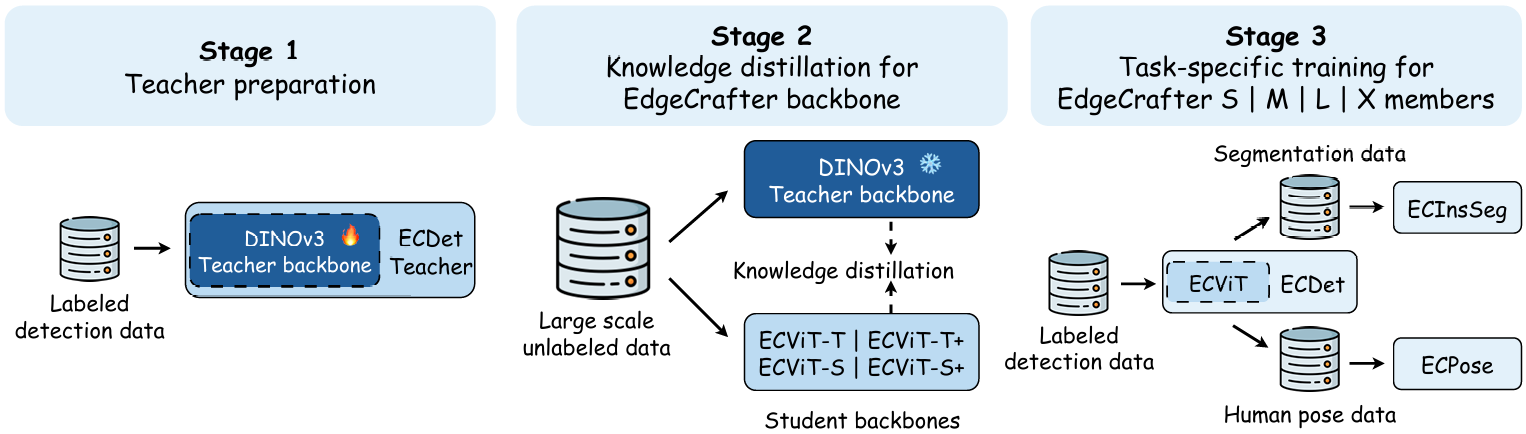
\includegraphics[width=\textwidth]{content/figures/edgecrafter_training.png}
\caption{Three-stage EdgeCrafter training pipeline. \cite{edgecrafter}}
\label{fig:edgecrafter_training}
\end{figure}

The training procedure consists of three stages \cite{edgecrafter}:

\begin{enumerate} \item \textbf{Teacher preparation:} A large DINOv3-pretrained Vision Transformer is first adapted to object detection, creating a task-specialized teacher model referred to as ECDet Teacher.

\item \textbf{Knowledge distillation:} The teacher's feature representations are distilled to compact \emph{ECViT} student backbones through feature alignment on a large image collection.

\item \textbf{Task-specific training:} The distilled student backbone is subsequently used to train \emph{ECDet}, \emph{ECInsSeg}, and \emph{ECPose} for their respective downstream tasks.

\end{enumerate}

The authors emphasize that object detection serves as the primary representation-learning task. The learned detection-oriented representations are then transferred directly to instance segmentation and human pose estimation through task-specific prediction modules \cite{edgecrafter}. Experimental results reported in the paper indicate that this task-specialized distillation strategy substantially improves downstream performance compared to conventional generic pretraining approaches.

\subsection{Architecture}

Figure~\ref{fig:edgecrafter_architecture} illustrates the overall ECDet architecture. The model consists of three main components: a compact transformer backbone ECViT, followed by an encoder and a decoder for set-based object prediction \cite{edgecrafter}.

\begin{figure}[htbp]
\centering
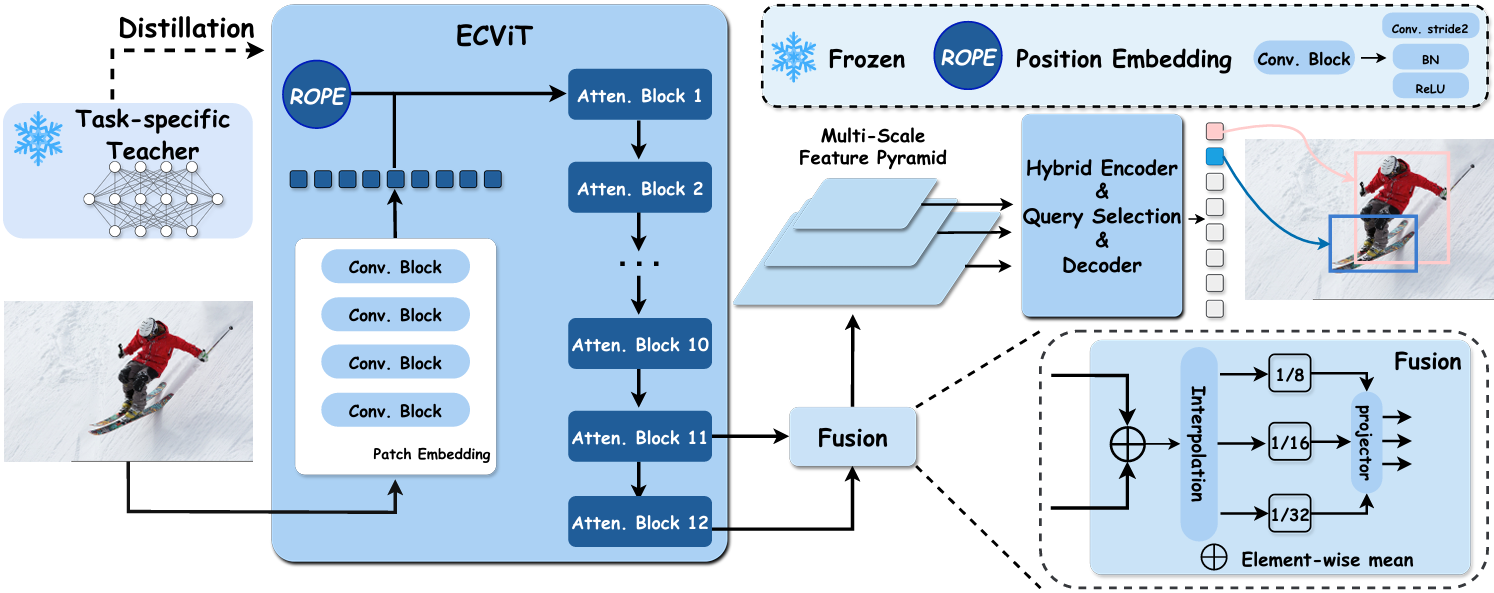
\includegraphics[width=\textwidth]{content/figures/edgecrafter_architecture.png}
\caption{Overview of the ECDet architecture. \cite{edgecrafter}}
\label{fig:edgecrafter_architecture}
\end{figure}

A key modification compared to conventional Vision Transformers is the replacement of the standard patch embedding layer with a lightweight convolutional stem consisting of four convolutional layers. According to the authors, this design preserves local image structures more effectively and improves dense localization performance. The generated feature representation is subsequently processed by a sequence of transformer attention blocks forming the EC\acrshort{vit} backbone. \cite{edgecrafter}

Since Vision Transformers do not naturally provide hierarchical feature pyramids, EdgeCrafter explicitly constructs a multi-scale feature representation from the final transformer layers. Rather than employing computationally expensive feature pyramid networks, the model generates feature maps at multiple resolutions using interpolation and lightweight convolutional projection layers. The resulting multi-scale feature representations are subsequently processed by an object detection head consisting of an encoder and a decoder. Following the design choices of RT-DETR, EdgeCrafter adopts a multi-scale hybrid encoder for feature aggregation and query selection. The decoder follows the DETR paradigm and predicts object classes and bounding boxes directly from the selected object queries. All three variants share the same distilled backbone representation and differ only in their lightweight task-specific prediction heads \cite{edgecrafter}.

\subsection{Performance Compared to State-of-the-Art Methods}

A major contribution of EdgeCrafter is its strong accuracy-efficiency trade-off. Figure~\ref{fig:edgecrafter_performance} compares the object detection performance of ECDet with several state-of-the-art detectors, including RT-DETRv4, RF-DETR, and YOLO26 \cite{edgecrafter}.

\begin{figure}[htbp]
\centering
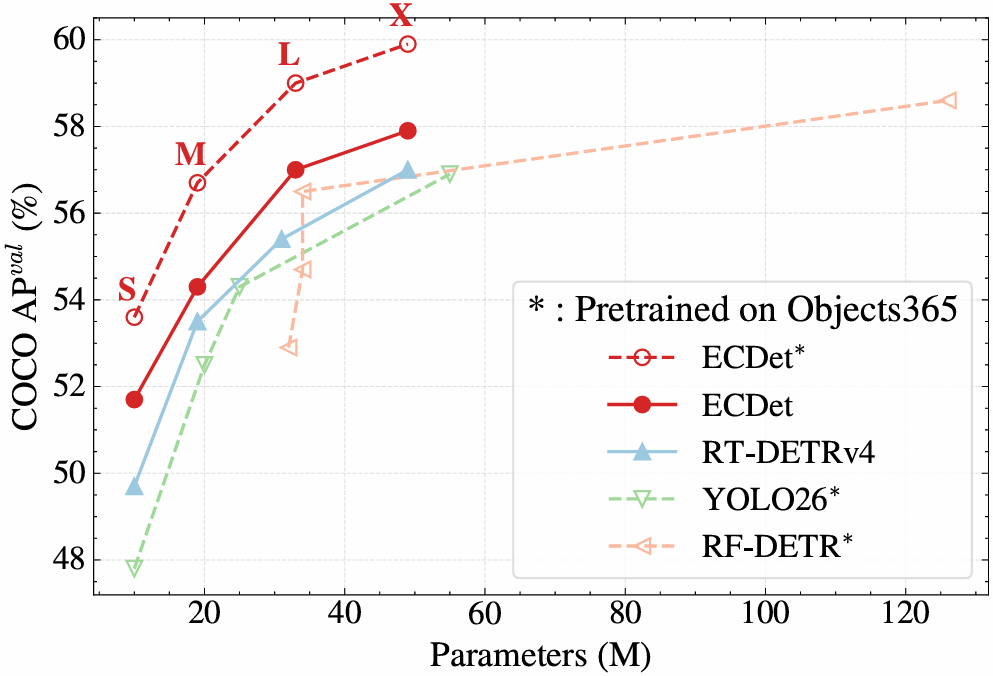
\includegraphics[width=0.75\textwidth]{content/figures/edgecrafter_result.png}
\caption{Comparison of COCO object detection performance and model size. Methods marked with * are pretrained on Objects365. \cite{edgecrafter}} \label{fig:edgecrafter_performance}
\end{figure}

The results demonstrate that ECDet achieves a favorable balance between model size and detection accuracy. For example, the smallest ECDet variant achieves 51.7 AP on the COCO validation dataset while using 10 million parameters. With additional Objects365 pretraining, ECDet-S reaches 53.6 AP. Compared to YOLO26-S, ECDet-S achieves higher detection performance at a comparable parameter count. The EdgeCrafter benchmark additionally reports competitive or superior performance compared to RT-DETRv4 and several other recent transformer-based detectors across multiple model scales. Similar observations are reported for the instance segmentation and human pose estimation variants ECInsSeg and ECPose, indicating that the distilled backbone transfers effectively across multiple dense prediction tasks. \cite{edgecrafter}

Overall, the results presented by Liu et al. suggest that compact Vision Transformers can achieve state-of-the-art performance in edge dense prediction when combined with task-specialized distillation and an architecture specifically designed for efficiency-constrained deployment scenarios \cite{edgecrafter}.
\chapter{Methodology}
\label{ch:methodology}

\section{Overview}
The repository documents several object detection experiments that are evaluated on a shared training and validation split. According to the experiment notes, all models are trained on the same training dataset and the metrics are computed on the validation set with the RailBench Toolkit.

\section{Model Variants}
The experiments cover YOLOv11-based baselines as well as EdgeCrafter-based detector variants. The YOLO notes include runs with no augmentation, blur augmentation, basic augmentation, and SAHI-based variants. The EdgeCrafter notes document ECDet configurations and a hybrid strategy that combines direct inference with SAHI inference.

\section{Implementation}
Representative YOLO runs use \texttt{yolo11s}, 300 epochs, a batch size of 12, an input size of 1024, and a fixed seed of 42. The EdgeCrafter runs use ECDet with AdamW, a flat-cosine learning-rate schedule, and 640-pixel evaluation resolution. These settings are reported here as project documentation rather than as a general prescription.

\chapter{Evaluations}
\label{ch:evaluations}

\section{Dataset}
The exploratory data analysis in the repository reports good data quality: there are no missing values, no NaNs, and no invalid bounding boxes. Most validation and test images are high-resolution, especially 3840\,$\times$\,2160 and 4112\,$\times$\,2504. The annotations are class-imbalanced, with \texttt{catenary\_pole} as the most frequent class and \texttt{train} and \texttt{bicycle} among the rarest classes. The bounding boxes are mostly small relative to the image size, show a strong height-to-width imbalance, and the data also contains occlusions and varying weather conditions.

\section{Metrics}
The experiment logs report average precision and recall-based metrics, including AP, AP50, AP75, APeasy, APmoderate, APhard, and the corresponding AR measures. For class-wise analysis, the logs also list AP values for individual classes across IoU thresholds from 0.50 to 0.95.

\section{Experimental Protocol}
All documented model runs use the same train/validation split and evaluate on the validation set with the RailBench Toolkit. This makes the runs directly comparable within the repository. The notes also distinguish between direct inference, SAHI inference, and a hybrid setup that merges predictions from both pipelines.

\section{Results}
The reported results show that augmentation and inference strategy matter for this benchmark. In the YOLO experiments, the no-augmentation baseline reaches AP 0.1460, while the blur-augmentation run improves to AP 0.1696. For EdgeCrafter, the hybrid direct-plus-SAHI configuration achieves AP 0.2968 and AP50 0.5429 on the validation set. Taken together, the results suggest that the benchmark is sensitive to small objects and class imbalance, and that SAHI-based or hybrid inference strategies can be beneficial.

\chapter{Conclusion}
\label{ch:conclusion}
In this project, we investigated different object detection approaches for the RAIL-BENCH Object Detection Challenge, focusing on the detection of small objects.
We evaluated \acrshort{yolo}11 and EdgeCrafter models using different training and inference strategies, such as sliced training, \acrshort{sahi} inference, and oversampling. In addition, we introduced a hybrid inference approach.

Our experiments showed that basic augmentation improved the \acrshort{yolo}11 baseline, while additional blur augmentations did not provide further benefits. Training on sliced images and using \acrshort{sahi} inference substantially improved detection performance, especially for smaller infrastructure objects such as catenary poles and signal poles.
Further improvements were achieved by increasing model capacity and input resolution.
ECDet-L achieved better results than the \acrshort{yolo}11 models, reaching 31.86\% AP hard with sliced training and \acrshort{sahi} inference.
However, \acrshort{sahi} inference was not beneficial for all object classes. In particular, train detection performed considerably better with direct inference, while smaller infrastructure objects benefited from slicing.
Our simple oversampling strategy did not improve overall detection performance in the tested configurations. This suggests that duplicating entire images may not be an effective way to address class imbalance.

Based on these observations, we developed a hybrid inference approach that combines predictions from a model trained on full images with predictions from a model trained on sliced images. This approach achieved the best validation result of 36.02\% AP hard, outperforming direct inference and \acrshort{sahi}-only inference.

Our final submission achieved 34.19 \% AP hard on the RAIL-BENCH test set, placing first among three submissions as of November 12, 2026. The difference between validation and test performance was relatively small, suggesting that the approach maintained much of its performance on unseen images.

The hybrid approach could potentially be improved by enhancing the selection of the inference strategy. For this specific use case, road vehicles might also perform better with direct inference, while in general, data-driven methods could be used to identify the best inference strategy for each class algorithmically.
Moreover, further work could investigate more targeted oversampling strategies that specifically address underrepresented objects.

Overall, our results demonstrate that combining sliced and full-image inference can improve railway object detection by exploiting the strengths of both approaches. In particular, the class-specific differences show that a single inference strategy is not necessarily optimal for all object categories.



%% Do not change, auto-generated lists of figures, tables and literature %%
% Glossar
\printunsrtglossary[type=abbreviations]
\cleardoublepage

% List of figures
\addcontentsline{toc}{chapter}{\listfigurename}
\listoffigures
\cleardoublepage

% List of tables
\addcontentsline{toc}{chapter}{\listtablename}
\listoftables
\cleardoublepage

% Literature list
% %CONFIG:
%\selectlanguage{german}{\addcontentsline{toc}{chapter}{\bibname}}
\selectlanguage{english}{\addcontentsline{toc}{chapter}{\bibname}}

\printbibliography
\end{document}
